% Options for packages loaded elsewhere
% Options for packages loaded elsewhere
\PassOptionsToPackage{unicode}{hyperref}
\PassOptionsToPackage{hyphens}{url}
\PassOptionsToPackage{dvipsnames,svgnames,x11names}{xcolor}
%
\documentclass[
  letterpaper,
  DIV=11,
  numbers=noendperiod]{scrartcl}
\usepackage{xcolor}
\usepackage{amsmath,amssymb}
\setcounter{secnumdepth}{-\maxdimen} % remove section numbering
\usepackage{iftex}
\ifPDFTeX
  \usepackage[T1]{fontenc}
  \usepackage[utf8]{inputenc}
  \usepackage{textcomp} % provide euro and other symbols
\else % if luatex or xetex
  \usepackage{unicode-math} % this also loads fontspec
  \defaultfontfeatures{Scale=MatchLowercase}
  \defaultfontfeatures[\rmfamily]{Ligatures=TeX,Scale=1}
\fi
\usepackage{lmodern}
\ifPDFTeX\else
  % xetex/luatex font selection
\fi
% Use upquote if available, for straight quotes in verbatim environments
\IfFileExists{upquote.sty}{\usepackage{upquote}}{}
\IfFileExists{microtype.sty}{% use microtype if available
  \usepackage[]{microtype}
  \UseMicrotypeSet[protrusion]{basicmath} % disable protrusion for tt fonts
}{}
\makeatletter
\@ifundefined{KOMAClassName}{% if non-KOMA class
  \IfFileExists{parskip.sty}{%
    \usepackage{parskip}
  }{% else
    \setlength{\parindent}{0pt}
    \setlength{\parskip}{6pt plus 2pt minus 1pt}}
}{% if KOMA class
  \KOMAoptions{parskip=half}}
\makeatother
% Make \paragraph and \subparagraph free-standing
\makeatletter
\ifx\paragraph\undefined\else
  \let\oldparagraph\paragraph
  \renewcommand{\paragraph}{
    \@ifstar
      \xxxParagraphStar
      \xxxParagraphNoStar
  }
  \newcommand{\xxxParagraphStar}[1]{\oldparagraph*{#1}\mbox{}}
  \newcommand{\xxxParagraphNoStar}[1]{\oldparagraph{#1}\mbox{}}
\fi
\ifx\subparagraph\undefined\else
  \let\oldsubparagraph\subparagraph
  \renewcommand{\subparagraph}{
    \@ifstar
      \xxxSubParagraphStar
      \xxxSubParagraphNoStar
  }
  \newcommand{\xxxSubParagraphStar}[1]{\oldsubparagraph*{#1}\mbox{}}
  \newcommand{\xxxSubParagraphNoStar}[1]{\oldsubparagraph{#1}\mbox{}}
\fi
\makeatother

\usepackage{color}
\usepackage{fancyvrb}
\newcommand{\VerbBar}{|}
\newcommand{\VERB}{\Verb[commandchars=\\\{\}]}
\DefineVerbatimEnvironment{Highlighting}{Verbatim}{commandchars=\\\{\}}
% Add ',fontsize=\small' for more characters per line
\usepackage{framed}
\definecolor{shadecolor}{RGB}{241,243,245}
\newenvironment{Shaded}{\begin{snugshade}}{\end{snugshade}}
\newcommand{\AlertTok}[1]{\textcolor[rgb]{0.68,0.00,0.00}{#1}}
\newcommand{\AnnotationTok}[1]{\textcolor[rgb]{0.37,0.37,0.37}{#1}}
\newcommand{\AttributeTok}[1]{\textcolor[rgb]{0.40,0.45,0.13}{#1}}
\newcommand{\BaseNTok}[1]{\textcolor[rgb]{0.68,0.00,0.00}{#1}}
\newcommand{\BuiltInTok}[1]{\textcolor[rgb]{0.00,0.23,0.31}{#1}}
\newcommand{\CharTok}[1]{\textcolor[rgb]{0.13,0.47,0.30}{#1}}
\newcommand{\CommentTok}[1]{\textcolor[rgb]{0.37,0.37,0.37}{#1}}
\newcommand{\CommentVarTok}[1]{\textcolor[rgb]{0.37,0.37,0.37}{\textit{#1}}}
\newcommand{\ConstantTok}[1]{\textcolor[rgb]{0.56,0.35,0.01}{#1}}
\newcommand{\ControlFlowTok}[1]{\textcolor[rgb]{0.00,0.23,0.31}{\textbf{#1}}}
\newcommand{\DataTypeTok}[1]{\textcolor[rgb]{0.68,0.00,0.00}{#1}}
\newcommand{\DecValTok}[1]{\textcolor[rgb]{0.68,0.00,0.00}{#1}}
\newcommand{\DocumentationTok}[1]{\textcolor[rgb]{0.37,0.37,0.37}{\textit{#1}}}
\newcommand{\ErrorTok}[1]{\textcolor[rgb]{0.68,0.00,0.00}{#1}}
\newcommand{\ExtensionTok}[1]{\textcolor[rgb]{0.00,0.23,0.31}{#1}}
\newcommand{\FloatTok}[1]{\textcolor[rgb]{0.68,0.00,0.00}{#1}}
\newcommand{\FunctionTok}[1]{\textcolor[rgb]{0.28,0.35,0.67}{#1}}
\newcommand{\ImportTok}[1]{\textcolor[rgb]{0.00,0.46,0.62}{#1}}
\newcommand{\InformationTok}[1]{\textcolor[rgb]{0.37,0.37,0.37}{#1}}
\newcommand{\KeywordTok}[1]{\textcolor[rgb]{0.00,0.23,0.31}{\textbf{#1}}}
\newcommand{\NormalTok}[1]{\textcolor[rgb]{0.00,0.23,0.31}{#1}}
\newcommand{\OperatorTok}[1]{\textcolor[rgb]{0.37,0.37,0.37}{#1}}
\newcommand{\OtherTok}[1]{\textcolor[rgb]{0.00,0.23,0.31}{#1}}
\newcommand{\PreprocessorTok}[1]{\textcolor[rgb]{0.68,0.00,0.00}{#1}}
\newcommand{\RegionMarkerTok}[1]{\textcolor[rgb]{0.00,0.23,0.31}{#1}}
\newcommand{\SpecialCharTok}[1]{\textcolor[rgb]{0.37,0.37,0.37}{#1}}
\newcommand{\SpecialStringTok}[1]{\textcolor[rgb]{0.13,0.47,0.30}{#1}}
\newcommand{\StringTok}[1]{\textcolor[rgb]{0.13,0.47,0.30}{#1}}
\newcommand{\VariableTok}[1]{\textcolor[rgb]{0.07,0.07,0.07}{#1}}
\newcommand{\VerbatimStringTok}[1]{\textcolor[rgb]{0.13,0.47,0.30}{#1}}
\newcommand{\WarningTok}[1]{\textcolor[rgb]{0.37,0.37,0.37}{\textit{#1}}}

\usepackage{longtable,booktabs,array}
\usepackage{calc} % for calculating minipage widths
% Correct order of tables after \paragraph or \subparagraph
\usepackage{etoolbox}
\makeatletter
\patchcmd\longtable{\par}{\if@noskipsec\mbox{}\fi\par}{}{}
\makeatother
% Allow footnotes in longtable head/foot
\IfFileExists{footnotehyper.sty}{\usepackage{footnotehyper}}{\usepackage{footnote}}
\makesavenoteenv{longtable}
\usepackage{graphicx}
\makeatletter
\newsavebox\pandoc@box
\newcommand*\pandocbounded[1]{% scales image to fit in text height/width
  \sbox\pandoc@box{#1}%
  \Gscale@div\@tempa{\textheight}{\dimexpr\ht\pandoc@box+\dp\pandoc@box\relax}%
  \Gscale@div\@tempb{\linewidth}{\wd\pandoc@box}%
  \ifdim\@tempb\p@<\@tempa\p@\let\@tempa\@tempb\fi% select the smaller of both
  \ifdim\@tempa\p@<\p@\scalebox{\@tempa}{\usebox\pandoc@box}%
  \else\usebox{\pandoc@box}%
  \fi%
}
% Set default figure placement to htbp
\def\fps@figure{htbp}
\makeatother





\setlength{\emergencystretch}{3em} % prevent overfull lines

\providecommand{\tightlist}{%
  \setlength{\itemsep}{0pt}\setlength{\parskip}{0pt}}



 


\KOMAoption{captions}{tableheading}
\makeatletter
\@ifpackageloaded{caption}{}{\usepackage{caption}}
\AtBeginDocument{%
\ifdefined\contentsname
  \renewcommand*\contentsname{Table of contents}
\else
  \newcommand\contentsname{Table of contents}
\fi
\ifdefined\listfigurename
  \renewcommand*\listfigurename{List of Figures}
\else
  \newcommand\listfigurename{List of Figures}
\fi
\ifdefined\listtablename
  \renewcommand*\listtablename{List of Tables}
\else
  \newcommand\listtablename{List of Tables}
\fi
\ifdefined\figurename
  \renewcommand*\figurename{Figure}
\else
  \newcommand\figurename{Figure}
\fi
\ifdefined\tablename
  \renewcommand*\tablename{Table}
\else
  \newcommand\tablename{Table}
\fi
}
\@ifpackageloaded{float}{}{\usepackage{float}}
\floatstyle{ruled}
\@ifundefined{c@chapter}{\newfloat{codelisting}{h}{lop}}{\newfloat{codelisting}{h}{lop}[chapter]}
\floatname{codelisting}{Listing}
\newcommand*\listoflistings{\listof{codelisting}{List of Listings}}
\makeatother
\makeatletter
\makeatother
\makeatletter
\@ifpackageloaded{caption}{}{\usepackage{caption}}
\@ifpackageloaded{subcaption}{}{\usepackage{subcaption}}
\makeatother
\usepackage{bookmark}
\IfFileExists{xurl.sty}{\usepackage{xurl}}{} % add URL line breaks if available
\urlstyle{same}
\hypersetup{
  pdftitle={Nora project},
  pdfauthor={Nora},
  colorlinks=true,
  linkcolor={blue},
  filecolor={Maroon},
  citecolor={Blue},
  urlcolor={Blue},
  pdfcreator={LaTeX via pandoc}}


\title{Nora project}
\author{Nora}
\date{}
\begin{document}
\maketitle


\subsection{Quarto}\label{quarto}

Quarto enables you to weave together content and executable code into a
finished document. To learn more about Quarto see
\url{https://quarto.org}.

\subsection{Running Code}\label{running-code}

When you click the \textbf{Render} button a document will be generated
that includes both content and the output of embedded code. You can
embed code like this:

\begin{Shaded}
\begin{Highlighting}[]
\NormalTok{melbh }\OtherTok{\textless{}{-}} \FunctionTok{read.csv}\NormalTok{(}\StringTok{"../../data\_sources/melb\_data.csv"}\NormalTok{)}
\FunctionTok{names}\NormalTok{(melbh)}
\end{Highlighting}
\end{Shaded}

\begin{verbatim}
 [1] "X"             "Suburb"        "Address"       "Rooms"        
 [5] "Type"          "Price"         "Method"        "SellerG"      
 [9] "Date"          "Distance"      "Postcode"      "Bedroom2"     
[13] "Bathroom"      "Car"           "Landsize"      "BuildingArea" 
[17] "YearBuilt"     "CouncilArea"   "Lattitude"     "Longtitude"   
[21] "Regionname"    "Propertycount"
\end{verbatim}

\begin{Shaded}
\begin{Highlighting}[]
\FunctionTok{str}\NormalTok{(melbh)}
\end{Highlighting}
\end{Shaded}

\begin{verbatim}
'data.frame':   13580 obs. of  22 variables:
 $ X            : int  1 2 3 4 5 6 7 8 9 10 ...
 $ Suburb       : chr  "Abbotsford" "Abbotsford" "Abbotsford" "Abbotsford" ...
 $ Address      : chr  "85 Turner St" "25 Bloomburg St" "5 Charles St" "40 Federation La" ...
 $ Rooms        : int  2 2 3 3 4 2 3 2 1 2 ...
 $ Type         : chr  "h" "h" "h" "h" ...
 $ Price        : num  1480000 1035000 1465000 850000 1600000 ...
 $ Method       : chr  "S" "S" "SP" "PI" ...
 $ SellerG      : chr  "Biggin" "Biggin" "Biggin" "Biggin" ...
 $ Date         : chr  "2016-12-03" "2016-02-04" "2017-03-04" "2017-03-04" ...
 $ Distance     : num  2.5 2.5 2.5 2.5 2.5 2.5 2.5 2.5 2.5 2.5 ...
 $ Postcode     : int  3067 3067 3067 3067 3067 3067 3067 3067 3067 3067 ...
 $ Bedroom2     : int  2 2 3 3 3 2 4 2 1 3 ...
 $ Bathroom     : int  1 1 2 2 1 1 2 1 1 1 ...
 $ Car          : int  1 0 0 1 2 0 0 2 1 2 ...
 $ Landsize     : int  202 156 134 94 120 181 245 256 0 220 ...
 $ BuildingArea : num  NA 79 150 NA 142 NA 210 107 NA 75 ...
 $ YearBuilt    : int  NA 1900 1900 NA 2014 NA 1910 1890 NA 1900 ...
 $ CouncilArea  : chr  "Yarra" "Yarra" "Yarra" "Yarra" ...
 $ Lattitude    : num  -37.8 -37.8 -37.8 -37.8 -37.8 ...
 $ Longtitude   : num  145 145 145 145 145 ...
 $ Regionname   : chr  "Northern Metropolitan" "Northern Metropolitan" "Northern Metropolitan" "Northern Metropolitan" ...
 $ Propertycount: int  4019 4019 4019 4019 4019 4019 4019 4019 4019 4019 ...
\end{verbatim}

\begin{Shaded}
\begin{Highlighting}[]
\FunctionTok{summary}\NormalTok{(melbh)}
\end{Highlighting}
\end{Shaded}

\begin{verbatim}
       X            Suburb            Address              Rooms       
 Min.   :    1   Length:13580       Length:13580       Min.   : 1.000  
 1st Qu.: 3396   Class :character   Class :character   1st Qu.: 2.000  
 Median : 6790   Mode  :character   Mode  :character   Median : 3.000  
 Mean   : 6790                                         Mean   : 2.938  
 3rd Qu.:10185                                         3rd Qu.: 3.000  
 Max.   :13580                                         Max.   :10.000  
                                                                       
     Type               Price            Method            SellerG         
 Length:13580       Min.   :  85000   Length:13580       Length:13580      
 Class :character   1st Qu.: 650000   Class :character   Class :character  
 Mode  :character   Median : 903000   Mode  :character   Mode  :character  
                    Mean   :1075684                                        
                    3rd Qu.:1330000                                        
                    Max.   :9000000                                        
                                                                           
     Date              Distance        Postcode       Bedroom2     
 Length:13580       Min.   : 0.00   Min.   :3000   Min.   : 0.000  
 Class :character   1st Qu.: 6.10   1st Qu.:3044   1st Qu.: 2.000  
 Mode  :character   Median : 9.20   Median :3084   Median : 3.000  
                    Mean   :10.14   Mean   :3105   Mean   : 2.915  
                    3rd Qu.:13.00   3rd Qu.:3148   3rd Qu.: 3.000  
                    Max.   :48.10   Max.   :3977   Max.   :20.000  
                                                                   
    Bathroom          Car           Landsize         BuildingArea  
 Min.   :0.000   Min.   : 0.00   Min.   :     0.0   Min.   :    0  
 1st Qu.:1.000   1st Qu.: 1.00   1st Qu.:   177.0   1st Qu.:   93  
 Median :1.000   Median : 2.00   Median :   440.0   Median :  126  
 Mean   :1.534   Mean   : 1.61   Mean   :   558.4   Mean   :  152  
 3rd Qu.:2.000   3rd Qu.: 2.00   3rd Qu.:   651.0   3rd Qu.:  174  
 Max.   :8.000   Max.   :10.00   Max.   :433014.0   Max.   :44515  
                 NA's   :62                         NA's   :6450   
   YearBuilt    CouncilArea          Lattitude        Longtitude   
 Min.   :1196   Length:13580       Min.   :-38.18   Min.   :144.4  
 1st Qu.:1940   Class :character   1st Qu.:-37.86   1st Qu.:144.9  
 Median :1970   Mode  :character   Median :-37.80   Median :145.0  
 Mean   :1965                      Mean   :-37.81   Mean   :145.0  
 3rd Qu.:1999                      3rd Qu.:-37.76   3rd Qu.:145.1  
 Max.   :2018                      Max.   :-37.41   Max.   :145.5  
 NA's   :5375                                                      
  Regionname        Propertycount  
 Length:13580       Min.   :  249  
 Class :character   1st Qu.: 4380  
 Mode  :character   Median : 6555  
                    Mean   : 7454  
                    3rd Qu.:10331  
                    Max.   :21650  
                                   
\end{verbatim}

\begin{Shaded}
\begin{Highlighting}[]
\FunctionTok{library}\NormalTok{(dplyr)}
\end{Highlighting}
\end{Shaded}

\begin{verbatim}

Attaching package: 'dplyr'
\end{verbatim}

\begin{verbatim}
The following objects are masked from 'package:stats':

    filter, lag
\end{verbatim}

\begin{verbatim}
The following objects are masked from 'package:base':

    intersect, setdiff, setequal, union
\end{verbatim}

\begin{Shaded}
\begin{Highlighting}[]
\DocumentationTok{\#\#\#Removing NA from the data  }
  
\NormalTok{melb2 }\OtherTok{\textless{}{-}}\NormalTok{ melbh[}\FunctionTok{complete.cases}\NormalTok{(melbh),]}
\NormalTok{melbPRA }\OtherTok{\textless{}{-}} \FunctionTok{select}\NormalTok{(melb2, Price,Rooms,}\AttributeTok{age=}\NormalTok{YearBuilt)}
\end{Highlighting}
\end{Shaded}

\begin{Shaded}
\begin{Highlighting}[]
\FunctionTok{library}\NormalTok{(ggplot2)}
\end{Highlighting}
\end{Shaded}

You can add options to executable code like this

\begin{Shaded}
\begin{Highlighting}[]
\FunctionTok{ggplot}\NormalTok{(melbPRA,}
       \FunctionTok{aes}\NormalTok{(}\AttributeTok{y=}\NormalTok{Price,}\AttributeTok{x=}\NormalTok{age, }\AttributeTok{colour=}\NormalTok{age)) }\SpecialCharTok{+}
  \FunctionTok{geom\_point}\NormalTok{() }\SpecialCharTok{+}
  \FunctionTok{scale\_colour\_viridis\_c}\NormalTok{() }\SpecialCharTok{+}
  \FunctionTok{geom\_smooth}\NormalTok{()}
\end{Highlighting}
\end{Shaded}

\begin{verbatim}
`geom_smooth()` using method = 'gam' and formula = 'y ~ s(x, bs = "cs")'
\end{verbatim}

\begin{verbatim}
Warning: The following aesthetics were dropped during statistical transformation:
colour.
i This can happen when ggplot fails to infer the correct grouping structure in
  the data.
i Did you forget to specify a `group` aesthetic or to convert a numerical
  variable into a factor?
\end{verbatim}

\pandocbounded{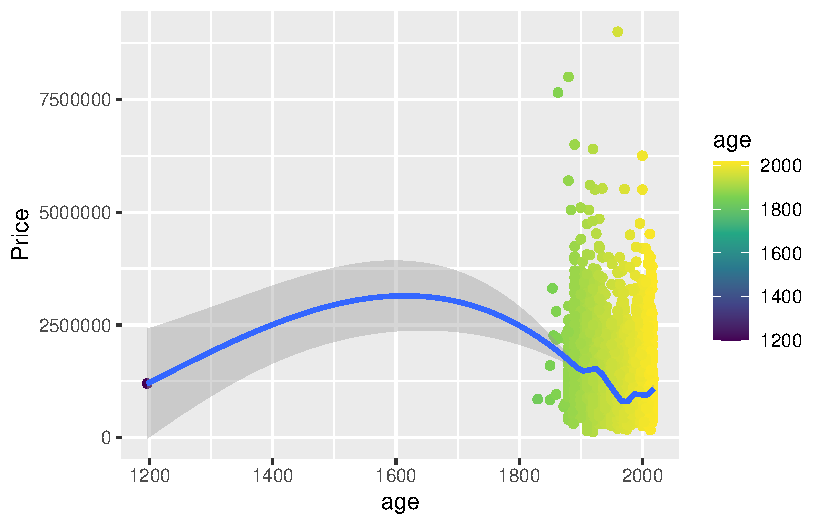
\includegraphics[keepaspectratio]{Nora-project_files/figure-pdf/unnamed-chunk-5-1.pdf}}

\begin{Shaded}
\begin{Highlighting}[]
\NormalTok{melbPRA }\OtherTok{\textless{}{-}}\NormalTok{ melbPRA }\SpecialCharTok{\%\textgreater{}\%} 
  \FunctionTok{filter}\NormalTok{(age}\SpecialCharTok{\textgreater{}}\DecValTok{1800}\NormalTok{)}
\end{Highlighting}
\end{Shaded}

The \texttt{echo:\ false} option disables the printing of code (only
output is displayed).

\begin{Shaded}
\begin{Highlighting}[]
\FunctionTok{cor}\NormalTok{(melbPRA}\SpecialCharTok{$}\NormalTok{Price,melbPRA}\SpecialCharTok{$}\NormalTok{age)}
\end{Highlighting}
\end{Shaded}

\begin{verbatim}
[1] -0.3165811
\end{verbatim}

\begin{Shaded}
\begin{Highlighting}[]
\NormalTok{melb\_model }\OtherTok{\textless{}{-}} \FunctionTok{lm}\NormalTok{(}\StringTok{"Price \textasciitilde{}age"}\NormalTok{, melbPRA)}

\NormalTok{b0 }\OtherTok{\textless{}{-}}\NormalTok{ melb\_model}\SpecialCharTok{$}\NormalTok{coefficients[}\DecValTok{1}\NormalTok{]}\CommentTok{\#intercept}
\NormalTok{b1 }\OtherTok{\textless{}{-}}\NormalTok{ melb\_model}\SpecialCharTok{$}\NormalTok{coefficients[}\DecValTok{2}\NormalTok{]}\CommentTok{\#slope}
\FunctionTok{ggplot}\NormalTok{(melbPRA,}
       \FunctionTok{aes}\NormalTok{(}\AttributeTok{y=}\NormalTok{Price,}\AttributeTok{x=}\NormalTok{age, }\AttributeTok{colour=}\NormalTok{age)) }\SpecialCharTok{+}
  \FunctionTok{geom\_point}\NormalTok{() }\SpecialCharTok{+}
  \FunctionTok{scale\_colour\_viridis\_c}\NormalTok{() }\SpecialCharTok{+}
  \FunctionTok{geom\_abline}\NormalTok{(}\AttributeTok{intercept=}\NormalTok{b0,}\AttributeTok{slope=}\NormalTok{b1)}
\end{Highlighting}
\end{Shaded}

\pandocbounded{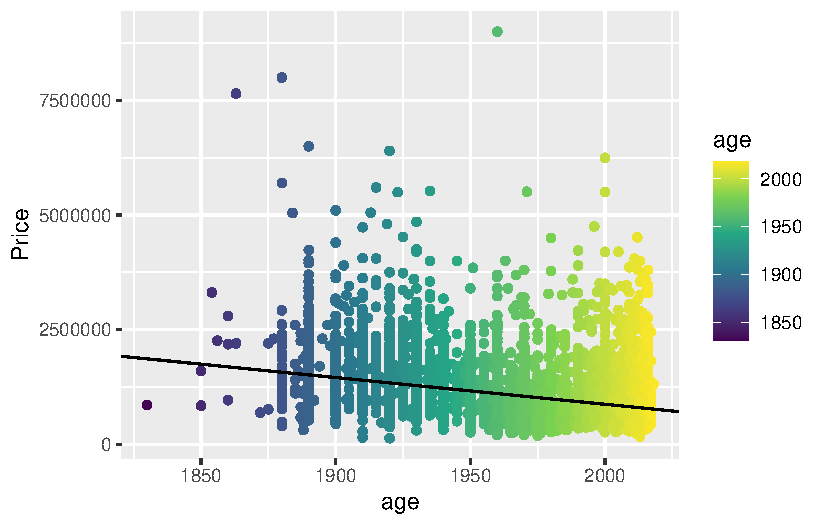
\includegraphics[keepaspectratio]{Nora-project_files/figure-pdf/unnamed-chunk-6-1.pdf}}




\end{document}
